\chapter{Neighbouring Problems}\label{ch:kacyang}\index{Kac, M.}\index{P\'olya, G.}\index{Yang, C. N.}\index{Lee Yang theorem}\index{Hilfssatz II}\index{Fisher zeros}

This chapter gathers problems next to the mass gap that share its mathematics. The first section takes from Kac and Yang a discrete system whose zeros can be located, and puts it in Thorin form (Chapter~\ref{ch:positivity}). The second reads stochastic quantisation and nonlinear filtering through the lattice Langevin equation and the Migdal Kadanoff ladder of Chapter~\ref{ch:strong}. The third reads our Hilbert sixth volume for what it says about the mass gap and what it supplies to the ladder. The last two take from our Riemann and Langlands volumes the tools, and the one negative result, that bear on this book.

\section{Kac, P\'olya and Yang: A Discrete System}

In the second volume of P\'olya's \emph{Collected Papers}, Mark Kac wrote a commentary~\cite{Ka74} on P\'olya's 1926 paper~\cite{Po26} on the integral representation of the Riemann $\xi$ function. It is three pages long. It records how a lemma from that paper, proved in pursuit of the Riemann Hypothesis, became an ingredient of the Lee and Yang circle theorem~\cite{LY52}, and it includes a recollection by C. N. Yang of the weeks in which the theorem was found. The Yang of that story is the Yang of Yang and Mills~\cite{YM54}, two years before their paper. This section tells the story, gives the mathematics, puts it in Thorin form following a 2026 note of the first author~\cite{Po26b}, and then does for Yang Mills what Kac did for the lattice gas: it looks at the smallest discrete system and asks where the zeros are.

\subsection{The commentary}

Kac begins by remarking that P\'olya's paper, though it comes very close to the Riemann Hypothesis, inspired little further work, and that it nevertheless played a small part in an important chapter of statistical mechanics. In late 1951 and early 1952 Lee and Yang were developing their theory of phase transitions and had been led, by examples, to a conjecture. For spins $\mu_k=\pm1$ and couplings $J_{kl}\ge0$, the function
\[
G_N(z)=\sum_{\mu}\exp\Big(\sum_{k,l=1}^NJ_{kl}\mu_k\mu_l\Big)\exp\Big(iz\sum_{k=1}^N\mu_k\Big)
\]
has only real zeros. When Kac heard of it he tried the simplest case, all couplings equal, and the second auxiliary theorem of P\'olya's paper, Hilfssatz II, came to his mind. He proved the conjecture in that case and showed the proof to Lee and Yang, who a couple of weeks later had the general theorem.

Yang's recollection, which Kac prints, fills in the rest. After about six weeks of failed attempts Kac showed them the equal coupling proof in early December, and around the twentieth Yang saw that by treating the fugacities of the sites as independent variables and following their motion relative to the unit circle, an induction of the same kind as Kac's would give everything. He calls the theorem ``a minor gem''~\cite[pp.~424 to 426]{Ka74}.

\subsection{Kac's proof}

Take $J_{kl}=\nu/2$ for all $k,l$, with $\nu>0$. Then the exponent depends on the spins only through $M=\sum\mu_k$, and adding one spin gives $\frac\nu2(M+\mu)^2+iz(M+\mu)=\frac\nu2M^2+(\nu\mu+iz)M+iz\mu+\frac\nu2$. Summing over the new spin,
\[
e^{-\nu/2}\,G_{N+1}(z)=e^{iz}\,G_N(z-i\nu)+e^{-iz}\,G_N(z+i\nu).
\]
The right side is P\'olya's operator. Hilfssatz II states that if $G$ is entire of genus at most one, real on the real axis, with only real zeros, then $e^{iz}G(z-i\nu)+e^{-iz}G(z+i\nu)$ has only real zeros. The proof, in Kac's form: at a zero $z=x+iy$ of the right side, $|e^{2iz}|^2=|G_N(z+i\nu)/G_N(z-i\nu)|^2$. If $G_N$ has real zeros $\alpha_n$, its Hadamard product gives
\[
e^{-4y}=\prod_n\frac{(\alpha_n-x)^2+(y+\nu)^2}{(\alpha_n-x)^2+(y-\nu)^2}.
\]
For $y>0$ every factor on the right exceeds one and the left side is below one; for $y<0$ the reverse. So $y=0$. The induction starts at $N=1$, where $G_1(z)=2e^{\nu/2}\cos z$.

We shall call this Kac's argument, and the displayed identity Kac's identity. It is an induction on the size of a discrete system, its engine is an operator that preserves a class of functions defined by where their zeros lie, and the reality of the zeros is proved by a comparison of signs that uses only the positivity of $\nu$, the ferromagnetic sign of the coupling.

\subsection{From one variable to many}

Kac's identity needs equal couplings, because only then does the new spin couple to the old ones through the single variable $M$. Yang's step was to give every site its own variable. With $z_k$ the fugacity of site $k$,
\[
\Phi_N(z_1,\dots,z_N)=\sum_{\mathcal I\subset\{1,\dots,N\}}W(\mathcal I)\prod_{k\in \mathcal I}z_k
\]
is a polynomial of degree one in each variable, and the claim becomes that $\Phi_N$ does not vanish when all $|z_k|<1$. Kac's function is the diagonal, $G_N(\zeta)=e^{iN\zeta}\Phi_N(w,\dots,w)$ with $w=e^{-2i\zeta}$, and real $\zeta$ is the unit circle. Adding a site gives $\Phi_{N+1}=P_0+z_{N+1}P_1$ with $P_0$ and $P_1$ of the same form, and the induction closes by a contraction lemma for polynomials of degree one in each of two variables, in the form later isolated by Asano~\cite{As70}: if $c_0+c_1z_1+c_2z_2+c_3z_1z_2$ has no zeros with both $|z_i|>1$, then $c_0+c_3z$ has none with $|z|>1$ (the form with $|z|<1$ follows by inversion). In this reading the circle theorem is Hilfssatz II carried from the line to the disc and applied one variable at a time.

\subsection{The Thorin form}

The bridge to this book is a rotation. If $G$ is even, of order one, with real zeros $\pm\alpha_n$, then $\tilde G(\sigma)=G(i\sigma)$ has $\tilde G(\sigma)/\tilde G(0)=\prod_n(1+\sigma^2/\alpha_n^2)$, and, factor by factor,
\[
\frac{G(0)}{G(i\sqrt s)}=\prod_n\Big(1+\frac{s}{\alpha_n^2}\Big)^{-1}=\E\,e^{-sH},\qquad H=\sum_n\frac{\mathcal E_n}{\alpha_n^2},
\]
with $\mathcal E_n$ independent standard exponentials. The reciprocal is the Laplace transform of a generalized gamma convolution~\cite{Th77,Bo92} whose Thorin measure is the counting measure $\sum_n\delta_{\alpha_n^2}$ on the squared zeros.

\begin{theorem}[Frullani bridge; Polson~\cite{Po26b}]\label{thm:frullani}
For $G$ even, entire of order one, real on the real axis, with $G(0)\ne0$, the following are equivalent: all zeros of $G$ are real; for every $\nu>0$ the zeros of $e^{iz}G(z-i\nu)+e^{-iz}G(z+i\nu)$ are real; and $G(0)/G(i\sqrt s)$ is the Laplace transform of a generalized gamma convolution, extending without zeros to the plane cut along the negative axis.
\end{theorem}

In this chapter only the implications from real zeros of $G$ to the other two conditions are used: the second is Hilfssatz II and the third is the displayed product. The converse implication is taken from~\cite{Po26b}; its proof, which needs the limit $\nu\to0$, is not reproduced here.

Kac's comparison of signs and Bondesson's theorem~\cite{Bo92} that the Laplace transform of a generalized gamma convolution has no zeros off the cut are two faces of one fact: the logarithm of $\tilde G$ is an integral of $1-e^{-\sigma^2s}$ against a positive measure. For a finite system the measure is atomic and the analytic continuation degenerates to a sign comparison. The Riemann Hypothesis, in the form of our Riemann volumes, is the same statement for a function whose Thorin measure is not known to be positive: the unbounded analogue of the circle theorem, with the inductive step missing.

Yang Mills sits on the other side of this bridge: in lattice gauge theory positivity of the spectral measure is free, by reflection positivity, and Section~\ref{ch:routeB} used the same Frullani identity, in the form of the $2\sin^2$ lemma, to transport it to a positive Thorin density. What is hard there is the support. The two problems that Yang's name is attached to are the two halves of one dictionary.

\subsection{Yang Mills as a discrete system: one plaquette}

Follow Kac and take the smallest system. For one plaquette of SU(2) lattice gauge theory the partition function in the weight $e^{\beta\cos\theta}$ is
\[
Z(\beta)=\int e^{\beta\cos\theta}\,\mathrm d\mathrm{Haar}=\frac{2I_1(\beta)}{\beta}.
\]
It is an even entire function of the coupling. Its zeros in the complex coupling, the Fisher zeros, are at $\beta=\pm i\,j_{1,n}$, with $j_{1,n}=3.832,\,7.016,\,10.173,\dots$ the positive zeros of the Bessel function $J_1$: all on the imaginary axis. So $Z$ is in exactly the rotated P\'olya class of the last subsection, and the bridge applies.

\begin{proposition}\label{prop:hitting}
For $\lambda>0$,
\[
\frac{1}{Z(\sqrt{2\lambda})}=\frac{\sqrt{2\lambda}}{2I_1(\sqrt{2\lambda})}=\prod_{n\ge1}\Big(1+\frac{2\lambda}{j_{1,n}^2}\Big)^{-1}=\E\,e^{-\lambda T},
\]
where $T$ is the first time that Brownian motion in $\R^4$, started at the origin, hits the unit sphere $S^3$, which is the group SU(2). The law of $T$ is a generalized gamma convolution with Thorin measure $\sum_n\delta_{j_{1,n}^2/2}$.
\end{proposition}

\begin{proof}
The radial part of Brownian motion in $\R^4$ is a Bessel process of index $a=1$, and the Laplace transform of its hitting time of one, started at zero, is $(\sqrt{2\lambda})^a/(2^a\Gamma(a+1)I_a(\sqrt{2\lambda}))$, by the classical results of Ciesielski and Taylor~\cite{CT62} and of Kent~\cite{Ke78}. The product is the Hadamard factorisation of $I_1(x)/x$.
\end{proof}

The proposition is the plaquette analogue of Kac's observation. The reciprocal of the Yang Mills partition function of one plaquette, as a function of the squared coupling, is the Laplace transform of a hitting time: the time for Brownian motion in the flat space in which the group sits as the unit sphere to reach the group. The same holds for U(1), the unit circle in the plane, with $I_0$ and $j_{0,n}$, and for any sphere. The Biane, Pitman and Yor variable~\cite{BPY} $S_{\mathrm{BPY}}$ of Section~\ref{ch:mk}, with transform $\sqrt{2\lambda}/\sinh\sqrt{2\lambda}$, is the member of the family with index $\frac12$, the hitting time of the two sphere. For a disc of $A$ plaquettes the partition function is $Z^A$ and its reciprocal is the transform of a sum of $A$ independent copies of $T$.

\subsection{A discrete system with complex zeros: the torus}

A disc of $A$ plaquettes in two dimensions has partition function $Z^A$, with the same zeros as one plaquette, and no dynamics; its plaquettes are independent. The smallest two dimensional system that is not a product is the torus, where the partition function is a sum over the characters of the group,
\[
Z_A(\beta)=\sum_{n\ge1}\Big(\frac{2I_n(\beta)}{\beta}\Big)^A ,
\]
with $A$ the number of plaquettes. We located its zeros numerically (Figure~\ref{fig:fisher}).

\begin{figure}[t]
\centering
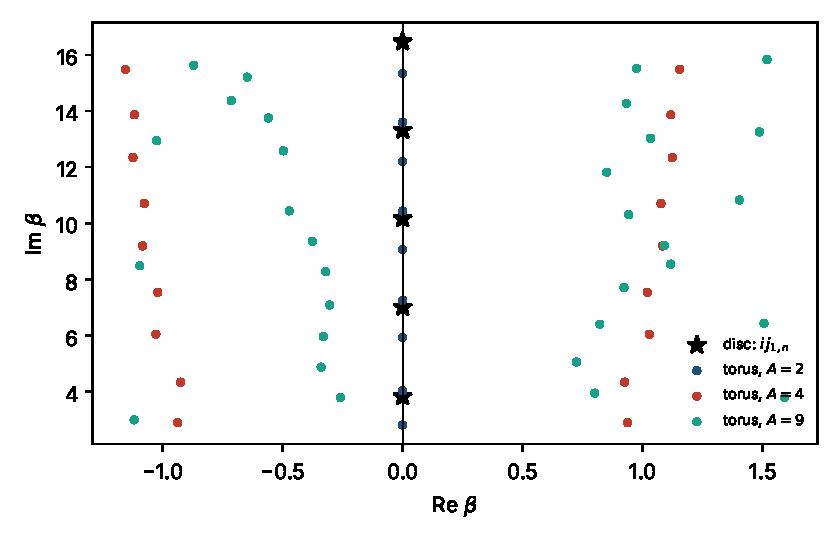
\includegraphics[width=0.55\textwidth]{figures/fisher_zeros.pdf}
\caption[Fisher zeros of two dimensional SU(2) lattice gauge theory]{Zeros in the upper half of the complex coupling plane of the partition function of two dimensional SU(2) lattice gauge theory: on a disc, where they lie on the imaginary axis at $i\,j_{1,n}$, and on tori of $2$, $4$ and $9$ plaquettes.}
\label{fig:fisher}
\end{figure}

For $A=2$ all zeros in the window $|\operatorname{Re}\beta|\le8$, $0<\operatorname{Im}\beta\le16$ lie on the imaginary axis. For $A=4$ and $A=9$ they do not: zeros appear with real parts up to $1.2$ and $1.6$. The closest to the real axis are at $-0.94+2.89i$ for $A=4$ and $-1.12+3.00i$ for $A=9$, against $3.83i$ for the disc. So the pure form of the property, all Fisher zeros imaginary, equivalently $Z(0)/Z(\sqrt s)$ the transform of a generalized gamma convolution, holds for the disc and, in the window searched, for the smallest torus, and fails for the larger tori computed. Nothing is wrong: in two dimensions the free energy per plaquette is $\log(2I_1(\beta)/\beta)$ in every infinite volume limit, analytic on the positive axis, and the zeros of the three tori we computed ($A=2$, $4$, $9$) stay a distance of about three from that axis. What the example shows is which form of the Lee and Yang property a gauge theory can be expected to have. It is not that the zeros lie on a line. It is that a neighbourhood of the positive real axis is free of zeros, uniformly in the volume.

In four dimensions that is the statement, assumed throughout this book, that there is no phase transition between strong and weak coupling; a Lee and Yang theorem for Yang Mills would be a proof that the Fisher zeros keep a fixed distance from the positive axis as the volume grows (Section~\ref{ch:missing}).

For the heat kernel action the question has an exact answer, and the reason is a scaling that Kac would have liked. On a torus of $A$ plaquettes with heat kernel weights $K_t$, the character coefficients are $e^{-(n^2-1)t/4}$, and
\[
Z_A(t)=\sum_{n\ge1}e^{-(n^2-1)At/4}=\mathcal G(q),\qquad q=e^{-At/4},
\]
where $\mathcal G(q)=1+q^3+q^8+q^{15}+\cdots=(\vartheta_3(q)-1)/(2q)$.
The partition function of every torus is one function of one variable.

\begin{theorem}[zeros on fixed rays]\label{thm:sector}
Let $q_1,q_2,\dots$ be the zeros of $\mathcal G$ in the unit disc and $s_j=-\log q_j$, with the principal logarithm. For two dimensional SU(2) lattice gauge theory with the heat kernel action on a torus of $A$ plaquettes, the zeros of the partition function in the complex time $t$, $\operatorname{Re}t>0$, are exactly $t=4(s_j+2\pi ik)/A$, $k\in\Z$. They lie on the same rays for every $A$, and $\mathcal G$ has no zeros in $|q|\le0.83$.
\end{theorem}

\begin{proof}
The identity for $Z_A$ is the definition, and $q=e^{-At/4}$ is a zero of $\mathcal G$ exactly when $At/4=s_j+2\pi ik$. For $|q|\le0.83$, $|\mathcal G(q)-1|\le|q|^3/(1-|q|^5)<1$.
\end{proof}

\paragraph{\normalfont\scshape A numerical result.} The sector $|\arg t|<\phi_*$, equivalently $|\arg\beta|<\phi_*$ for $\beta=2/t$, with $\phi_*=\inf_j|\arg s_j|$, contains no zero for any $A$. Numerically the zeros of $\mathcal G$ of smallest modulus are
\[
q_1=0.3888+0.7793\,i,\qquad q_2=-0.8669+0.2999\,i,
\]
with $|\arg s_1|=82.9^\circ$ and $|\arg s_2|=88.2^\circ$, so that $\phi_*=82.9^\circ$. The script \texttt{code/torus\_sector.py} counts the zeros of $\mathcal G$ by the argument principle on circles, finding $2$, $4$ and $82$ zeros in $|q|<0.9$, $0.95$ and $0.997$, and finds the same $41$ zeros in the upper half plane by Newton's method. In the closed sector the modular identity $\vartheta_3(e^{-s})=\sqrt{\pi/s}\,\vartheta_3(e^{-\pi^2/s})$ gives $|\vartheta_3(e^{-s})|\ge1.11$ for $|s|\le0.8$, and for $|s|\ge0.8$ the sector lies in $|q|\le0.906$, where $q_1$ and its conjugate are the only zeros. This is a floating point computation, not a certified one, and we do not call it a proof.

\begin{figure}[t]
\centering
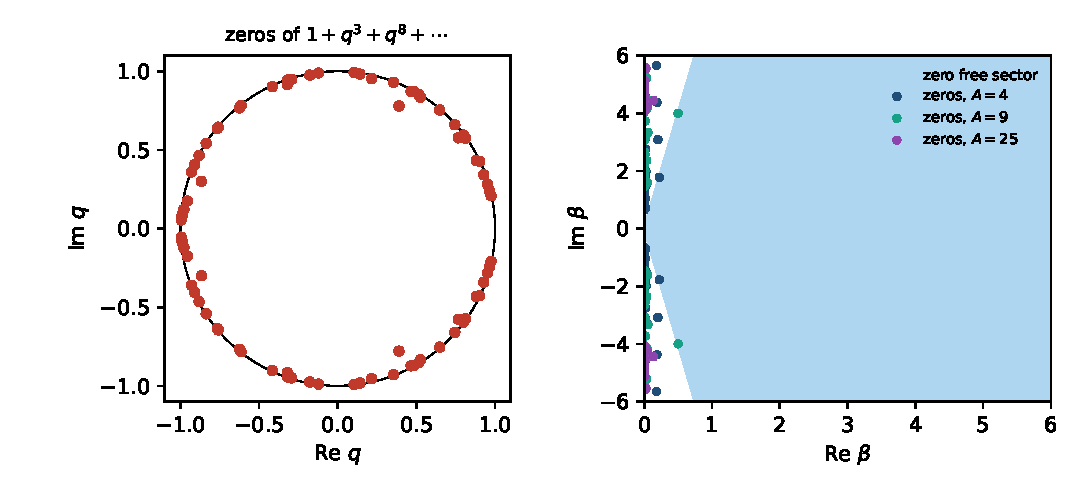
\includegraphics[width=0.75\textwidth]{figures/torus_sector.pdf}
\caption[A numerical zero free sector for the heat kernel torus]{Left: the zeros of $\mathcal G(q)=1+q^3+q^8+\cdots$ in the unit disc with $|q|\le0.997$. Right: the corresponding Fisher zeros in the coupling $\beta=2/t$ for tori of $4$, $9$ and $25$ plaquettes, all outside the sector of half angle $82.9^\circ$ around the positive axis.}
\label{fig:torussector}
\end{figure}

So for the heat kernel action in two dimensions the computation shows the Lee and Yang property in the form that matters: the zeros are confined, for every volume at once, to within about seven degrees of the imaginary axis (Figure~\ref{fig:torussector}), by a numerical value of the angle and not by a proof. The Wilson action lacks the scaling, and its zeros, shown in Figure~\ref{fig:fisher}, wander further.

\begin{problem}\label{op:neigh1}
Prove a zero free sector around the positive axis, uniform in the volume, for the Wilson action on two dimensional tori, and for the partition function on hierarchical lattices, where the Migdal Kadanoff recursion acts on the zeros as P\'olya's operator acts in Kac's proof.
\end{problem}

\subsection{What is due to Kac}

The observation that P\'olya's Hilfssatz II, a lemma about the Riemann $\xi$ function, proves a theorem of statistical mechanics is Kac's, and so is the proof of the circle theorem for equal couplings, the first proof of any case of it. The identity that compares $e^{-4y}$ with a product over the zeros, which the Frullani bridge identifies with the positivity of a Thorin measure, is his. And the method is his: when faced with a hard conjecture about a large system, take the smallest case, the most symmetric coupling, and a single variable, and find the mechanism there. Proposition~\ref{prop:hitting} and Theorem~\ref{thm:sector} are that method applied to one plaquette and to a torus.

The idea that organises our whole approach to four dimensions, that an exactly solvable caricature can carry the truth of a hard problem, is the thesis of his essay on models~\cite{Ka69}. This book treats the Migdal Kadanoff ladder as a caricature in exactly his sense.

Kac wrote his commentary to give credit to P\'olya for a paper that had been little noticed, and took care to print Yang's own account beside his. We have tried to follow that example.

\section{Stochastic Quantisation, Filtering and the Ladder}\label{ch:spde}\index{stochastic quantisation}\index{stochastic partial differential equation}\index{Hairer, M.}\index{regularity structures}\index{Zakai equation}\index{Kushner Stratonovich equation}\index{Kurtz, T. G.}\index{Xiong, J.}\index{particle filter}

Section~\ref{ch:probabilists} named the probabilists who work on gauge fields. We return to them with the rest of the book in hand, and ask of each line of work the question we have asked of everything else: what does it say about the gap? We have read the abstracts, introductions and statements of main results of the papers cited, not their proofs, and we report them at that level.

\subsection{The Langevin equation of a gauge field}\index{Parisi, G.}\index{Langevin dynamics}

Parisi and Wu~\cite{PW81} proposed in 1981 to construct a Euclidean field theory as the invariant law of a diffusion: the gradient flow of the action, driven by white noise in space and a fictitious time. For a gauge field $A$ with curvature $F_A$ the equation is
\[
\partial_\tau A=-D_A^*F_A+\xi ,
\]
with $\xi$ a space time white noise with values in the Lie algebra. Two things make it hard. The noise is rough, so that $A$ is a distribution and the quadratic and cubic terms of $D_A^*F_A$ are products of distributions; and the equation is covariant under gauge transformations, so that it is parabolic only after a gauge is fixed, by the device of DeTurck~\cite{DT83}.

On a lattice none of this is singular, and the equation is a system of interacting diffusions, one for each link:
\[
dU_\ell=-\tfrac\beta2\nabla_\ell S(U)\,d\tau+dB_\ell ,
\]
where $B_\ell$ are independent Brownian motions on the group and $\nabla_\ell S$ is the gradient of the Wilson action with respect to the link, a function of its staples. Its invariant law is the Wilson measure. It is a continuous time relative of the heat bath algorithm of Section~\ref{ch:latticemc}, with the same invariant law, and its spectral gap is the dynamic gap of Section~\ref{ch:dynamic}.

\subsection{What has been constructed}

\paragraph{\normalfont\scshape Two dimensions.} Chandra, Chevyrev, Hairer and Shen~\cite{CCHS} constructed the Langevin dynamic of the two dimensional Yang Mills measure on the torus with Hairer's regularity structures~\cite{Ha14}: a state space of distributional connections on which holonomies along smooth curves make sense, local solutions, and gauge covariance in law after renormalisation. Chevyrev and Shen~\cite{ChSh23} then proved that the two dimensional Yang Mills measure is invariant for the renormalised dynamic, for any connected compact structure group, by passing through the lattice and Bourgain's method~\cite{Bo96} for invariant measures, and derived a universality statement for lattice actions.

\paragraph{\normalfont\scshape Two dimensions with matter.} Bringmann, Cao, Hairer and Zhao~\cite{BCHZ} constructed the nonabelian Yang Mills Higgs measure on the two dimensional torus by stochastic quantisation alone. It holds for any fixed couplings. No rate of convergence and no mass gap is claimed.

\paragraph{\normalfont\scshape Three dimensions.} Chandra, Chevyrev, Hairer and Shen~\cite{CCHS3} defined a state space and a Markov process on gauge orbits for the stochastic quantisation of Yang Mills Higgs in three dimensions, up to a possible blow up in finite time, with a unique choice of counterterms that makes the solution gauge covariant in law. The measure in three dimensions has not been constructed this way.

\paragraph{\normalfont\scshape Four dimensions.} The equation is critical in four dimensions, in the sense of regularity structures, and no local theory exists. This is the stochastic face of asymptotic freedom: the nonlinearity is not small at small scales by power counting, only by a logarithm.

\subsection{One plaquette, exactly}\index{Bakry \'Emery criterion}

The dynamic route can be seen in full on the smallest example. Take one plaquette, that is one group element $U$ with law proportional to $e^{\beta\cos\theta}$ times Haar measure, and its Langevin equation with generator $L=\frac12\Delta+\frac\beta2\nabla\cos\theta\cdot\nabla$. On the unit sphere $S^3$ the Ricci curvature is $2$ and the Hessian of $a_0=\cos\theta$ is $-a_0$ times the metric, so the Bakry \'Emery~\cite{BE} curvature is
\[
\tfrac12\big(2+\beta\cos\theta\big)\ \ge\ 1-\frac\beta2 ,
\]
and the criterion gives a gap of at least $1-\beta/2$ for $\beta<2$ and nothing beyond. The true spectrum is easy to compute. The generator commutes with rotations about the identity, its eigenfunctions split by angular momentum $l$, and each sector is a Sturm Liouville problem in $\theta$.

\begin{center}
\small
\begin{tabular}{cccccccc}
\toprule
$\beta$ & 0 & 1 & 2 & 4 & 6 & 8 & 12 \\ \midrule
$l=0$ & 1.500 & 1.600 & 1.897 & 3.051 & 4.809 & 6.848 & 10.93 \\
$l=1$ & 1.500 & 1.566 & 1.758 & 2.439 & 3.337 & 4.304 & 6.282 \\
bound & 1.00 & 0.50 & 0.00 & $-1.00$ & $-2.00$ & $-3.00$ & $-5.00$ \\
\bottomrule
\end{tabular}
\end{center}
The rows are the lowest nonzero rate among class functions, the lowest rate in the sector $l=1$, which is the gap among the sectors computed (the sectors $l\ge2$ were not), and the Bakry \'Emery bound.

\begin{figure}[t]
\centering
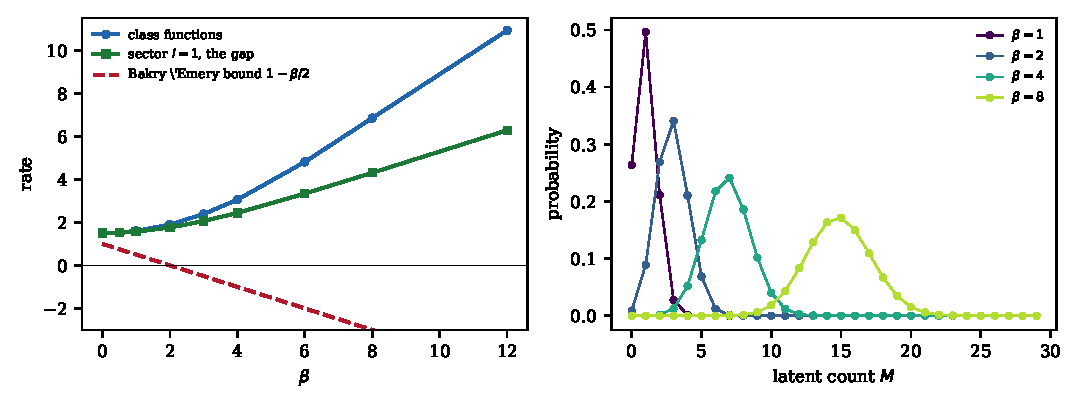
\includegraphics[width=0.75\textwidth]{figures/langevin_latent.pdf}
\caption[One plaquette Langevin gaps and the latent count]{Left: the spectral gap of the Langevin dynamic of one SU(2) plaquette in the sectors $l=0$ and $l=1$, and the Bakry \'Emery lower bound, which becomes void at $\beta=2$ while the gap grows. Right: the law of the latent count $M$ of Section~\ref{ch:langlands} for the heat kernel at four couplings.}
\label{fig:langevinlatent}
\end{figure}

The gap grows with $\beta$, like $\beta/2$, because near the identity the dynamic is an Ornstein Uhlenbeck process with that rate. The bound falls with $\beta$ and is void from $\beta=2$ on (Figure~\ref{fig:langevinlatent}). The reason is instructive. The bound is a minimum over the group, attained at the antipode, where the potential is concave. The measure gives the antipode weight of order $e^{-2\beta}$. So the criterion fails because of a region that the measure does not see.

This is the bad cap of Chapter~\ref{ch:progress} in another guise. There, total positivity of the convolution kernel failed in a cap at the antipode of small mass; here, uniform convexity fails in a cap at the same antipode. In both, a pointwise criterion is defeated by a set of negligible measure, and the remedy must be a criterion that averages, a Poincar\'e inequality proved by a Lyapunov function and a local inequality in the manner of Bakry, Cattiaux and Guillin~\cite{BCG08}. The single plaquette shows that the failure of the criterion is not evidence against a gap.

\subsection{What this says about the gap}

Two readings, in increasing order of relevance to this book.

First, the existence results are about the ultraviolet. They are the dynamic counterpart of Ba\l aban's stability bounds: control uniform in the cutoff at a fixed physical scale. The gap is an infrared statement. In our language, the stochastic quantisation programme constructs the measure and is silent, so far, on its support.

Second, where the dynamics has a gap, the measure has one. Shen, Zhu and Zhu~\cite{SZZ} proved on the lattice at strong coupling that the Langevin dynamic satisfies the Bakry \'Emery condition, hence a log Sobolev inequality uniform in the volume, hence exponential decay of correlations and a mass gap, with large $N$ consequences. This is the dynamic route of Section~\ref{ch:dynamic} carried out where curvature of the group beats the Hessian of the action. Cao, Nissim and Sheffield~\cite{CNS25} extended the regime in which the area law is proved for $U(N)$ lattice theories, in particular at large $N$, improving on Osterwalder and Seiler~\cite{OSe}, and gave a sufficient condition for the area law in terms of a strong enough mass gap; a companion paper takes a dynamical approach. The direction of that implication, from a gap to an area law, is the one this book has not used and should: our ladder gives the string tension first and the gap second.

Other work on the list of Section~\ref{ch:probabilists}: two dimensional Yang Mills as Brownian motion on the group indexed by area (Gross, King and Sengupta~\cite{GKS89}, Sengupta~\cite{Se97}, L\'evy~\cite{Le03}), on which everything exact in this book rests; Chatterjee's survey~\cite{Ch19}; and the surface expansions of Wilson loops of Cao, Park and Sheffield~\cite{CPS25}, whose signs are the obstruction to a probabilistic reading. The ground state representation of Proposition~\ref{prop:groundstate} is the picture of Nelson~\cite{Ne73} and Gross~\cite{Gro75} applied to a gauge field.

The stochastic quantisation programme and this book meet at one object, the lattice Langevin equation, and look at it from opposite ends. They take the lattice spacing to zero at fixed size and ask whether the dynamics survives. We fix the lattice, block it, and ask where the coupling goes. A proof of the gap would need both: their uniformity in the cutoff, and a statement like ours, on the real lattice, that blocking moves the effective law toward the region where the dynamics is known to contract.

\subsection{Filtering and the ladder in continuous scale}\label{ch:spdefilter}

There is a second family of stochastic equations, older in statistics, in which the unknown is a probability law: the equations of nonlinear filtering. The link is the interacting particle system, which is a numerical method for a filtering equation, by Kurtz and Xiong a representation of its solution, and, for a lattice gauge field, the Langevin equation itself. Chapter 20 of our Hilbert sixth book~\cite{PS26h} treats the filtering side; here we add what the gauge theory needs, and one formula, the ladder in continuous scale.

A signal $X_s$ diffuses with generator $L$ and is observed through $dY_s=h(X_s)\,ds+dV_s$. The unnormalised conditional density $\varrho_s$ of the signal given the observations solves Zakai's linear equation~\cite{Za69}, and the normalised law $\pi_s$ solves the nonlinear equation of Kushner and Stratonovich~\cite{Ku64,St60}:
\begin{align*}
d\varrho_s&=L^*\varrho_s\,ds+\varrho_s\,h\,dY_s,\\
d\pi_s(f)&=\pi_s(Lf)\,ds+\big(\pi_s(h f)-\pi_s(h)\pi_s(f)\big)\big(dY_s-\pi_s(h)\,ds\big).
\end{align*}
Two operations alternate, in continuous time: prediction by the Fokker Planck flow, and correction by a likelihood. The correction term is a covariance: the law moves in the direction in which $f$ is correlated with the log likelihood. A particle filter is the Monte Carlo form: move the particles by the signal dynamics, weight them by the likelihood, resample.

Kurtz and Xiong~\cite{KX99} turned the algorithm into a theorem: for an infinite exchangeable system of weighted particles sharing a common noise, the weighted empirical measure is the unique solution of a nonlinear stochastic partial differential equation in a class that contains the Zakai and Kushner Stratonovich equations, with the observation as common noise, and the McKean Vlasov equation, with no common noise. Later work gives error bounds~\cite{KX01}, Gaussian fluctuations~\cite{KX04} and boundary conditions~\cite{CJK18}.

The lattice Langevin equation is a system of interacting diffusions on the group with independent noises, no common noise and no exchangeability, only translation invariance, so the Kurtz Xiong theorem does not apply to it as it stands. We use the filtering equations as an analogy for the Migdal Kadanoff ladder, which is a filter in scale: Section~\ref{ch:plgbc} called bond moving the update and decimation the prediction. The next formula makes the scale continuous and finds the Kushner Stratonovich form exactly, without noise.

\index{beta function}
Let the scale factor be $b=1+d\varsigma$. Bond moving raises the density to the power $b^{d-2}=1+(d-2)\,d\varsigma$, and decimation takes the convolution power $b^2=1+2\,d\varsigma$. To first order in $d\varsigma$ the law $\rho_\varsigma$ of a link therefore satisfies
\[
\partial_\varsigma\rho=(d-2)\,\rho\,\big(\log\rho-\langle\log\rho\rangle_\rho\big)+2\,\mathcal C\rho ,
\]
where $\mathcal C\rho$ is the generator of convolution powers, which multiplies the character coefficient $u_n$ by $\log u_n$; on the heat kernel family $\mathcal C K_t=t\,\partial_tK_t$. This has the form of the Kushner Stratonovich equation with the noise removed, the innovation $dY_s-\pi_s(h)\,ds$ being replaced by $(d-2)\,d\varsigma$: the first term is a Bayes correction in which the law is its own likelihood, with rate $d-2$, and the second is a prediction. The correction term changes the mean of any $f$ at the rate $(d-2)\operatorname{Cov}_\rho(f,\log\rho)$.

\begin{proposition}[the projected ladder in continuous scale]\label{prop:contladder}
For SU(2), project onto the heat kernel family by the fundamental coefficient $u_2=e^{-3t/4}$ after each infinitesimal step. Then
\[
\frac{dt}{d\varsigma}=(4-d)\,t+(d-2)\,\mathcal B(t),\qquad\mathcal B(t)=t-\tfrac43e^{3t/4}\operatorname{Cov}_{K_t}\!\big(\cos\theta,\log K_t\big).
\]
\begin{enumerate}
\item[(i)] $\mathcal B(t)>0$ for every $t>0$.
\end{enumerate}
If the remainder in Theorem~\ref{thm:expansion} is $O((k-1)t^4)$, then
\begin{enumerate}
\item[(ii)] $\mathcal B(t)=\frac{t^2}6+\frac{t^3}{36}+\frac{t^4}{432}+O(t^5)$.
\item[(iii)] In four dimensions, with $\beta=2/t$, $\ \dfrac{d\beta}{d\varsigma}=-\dfrac23\Big(1+\dfrac1{3\beta}+\dfrac1{18\beta^2}+\cdots\Big)$.
\end{enumerate}
\end{proposition}

\begin{proof}
With $s(k)$ defined by $e^{-3s/4}=\int\cos\theta\,K_t^k/\int K_t^k$, differentiation at $k=1$ gives $s'(1)=-\frac43e^{3t/4}\operatorname{Cov}_{K_t}(\cos\theta,\log K_t)$. One step is $t\mapsto b^2s(b^{d-2})$, and expanding in $d\varsigma$ gives the formula. (i) Differentiating $e^{-3t/4}=\langle\cos\theta\rangle_{K_t}$ in $t$ gives $\frac34te^{-3t/4}=-\operatorname{Cov}_{K_t}(\cos\theta,t\,\partial_t\log K_t)$, so $\mathcal B(t)=-\frac43e^{3t/4}\operatorname{Cov}_{K_t}\big(\cos\theta,\partial_t(t\log K_t)\big)$. By Theorem~\ref{thm:scaledmlr} and Proposition~\ref{prop:initial}, $\partial_t(t\log K_t)$ is strictly decreasing in $\cos\theta$, and the covariance of an increasing and a strictly decreasing function of the same variable is negative. (ii) and (iii) are Theorem~\ref{thm:expansion} with $1-1/k=(d-2)\,d\varsigma$ and $k\to1$, which needs the $O(t^4)$ remainder there to be $O((k-1)t^4)$; the theorem does not state this, so (ii) and (iii) are conditional on it.
\end{proof}

On the real lattice the effective law of a block link depends on the neighbouring blocks, which is a common noise in the sense of Kurtz and Xiong; a stochastic ladder with such a noise is the natural extension, and we have not pursued it. The filtering form gives the ladder's beta function as a covariance, with the sign from Theorem~\ref{thm:scaledmlr}. None of it is a proof of the gap.

\section{Quantum Yang Mills and Hilbert's Sixth Problem}\label{ch:h6ym}\index{Hilbert's sixth problem}\index{Nelson, E.}\index{Feynman Kac formula}\index{ground state measure}\index{L\'evy area}\index{particle filter}\index{random walk on a group}

Our book \emph{On Hilbert's 6th Problem: Probability, Mechanics and Bayesian Computation}~\cite{PS26h} follows Hilbert's programme from Kolmogorov's axioms to the Navier Stokes equations and back, reading the inverse passage as Bayesian computation. Its last chapter contains a section on Yang Mills, written when the existence proof was announced, and several of its theorems are tools this book uses. Section and theorem numbers below refer to its version 1.1.0.

\subsection{Quantum field theory as a form of the sixth problem}

Hilbert asked in 1900 for a mathematical treatment of the axioms of physics, beginning with probability and mechanics. Its Section 9.6 places quantum field theory in the same frame: Wick rotation turns the Schr\"odinger group into the heat semigroup; Osterwalder and Schrader~\cite{OS} gave axioms for Euclidean Green functions in 1973, corrected in 1975 by a linear growth condition, under which the Euclidean theory continues to a relativistic one satisfying Wightman's axioms~\cite{SW64}; Nelson~\cite{Ne73} showed that Euclidean free fields are Markov fields; and Glimm and Jaffe~\cite{GJ} built interacting theories in two and three dimensions that way.

Quantum Yang Mills is that programme in its hardest case: existence was announced in 2026 and endorsed by a review group~\cite{OAI}, with ultraviolet stability by Ba\l aban~\cite{Ba87}, and the mass gap is the open statement about the long range behaviour of a measure whose short range behaviour is under control.

\subsection{Feynman Kac: the gap is a decay rate}

Theorem 9.4 of the Hilbert sixth book is the Feynman Kac formula: for $H=-\frac12\Delta+V$, the solution of the imaginary time equation is $\E_x\big[f(B_\tau)\exp(-\int_0^\tau V(B_s)\,\mathrm ds)\big]$. The ground state energy is the exponential decay rate of that expectation, and by the Donsker and Varadhan theory~\cite{DV75} a large deviation rate.

For Yang Mills in the Hamiltonian formulation of Kogut and Susskind~\cite{KS75}, the configuration space is a product of copies of SU(2), one for each spatial link, restricted to gauge invariant functions; the kinetic term is $g^2/(2a)$ times the sum of the quadratic Casimir operators of the group factors, each a Laplacian normalised to have eigenvalue $\frac34$ on the fundamental character; and the potential is a sum of spatial plaquette terms with a coefficient proportional to $1/(g^2a)$. In two spacetime dimensions there are no spatial plaquettes, the potential vanishes, the path measure is Brownian motion on the group, and the gap is the first eigenvalue of the Laplacian: the solution of Chapter~\ref{ch:twod}, read as the simplest case of Theorem 9.4.

The mass gap is the difference of two decay rates, $E_1-E_0$. Route B of this book is the statement that after the $2\sin^2$ transport that difference is itself a decay rate, of a positive Thorin density.

\subsection{Nelson: the gap is a Poincar\'e constant}

Section 9.5 of the Hilbert sixth book presents Nelson's stochastic mechanics~\cite{Ne66}: to a state $\psi$ corresponds a diffusion with drift $\nabla\log|\psi|$ and stationary law $|\psi|^2$, and its worked example, the harmonic oscillator, has the Ornstein Uhlenbeck process as the ground state diffusion. That picture gives a clean form of the mass gap.

\begin{proposition}[ground state representation]\label{prop:groundstate}
Let $H=-\frac{\kappa}{2}\Delta+V$ on a compact Riemannian manifold have a positive ground state $\Omega$ with energy $E_0$. The map $f\mapsto f\Omega$ carries $H-E_0$ on $L^2(\mathrm dx)$ to the operator
\[
L=-\frac\kappa2\Delta-\kappa\,\nabla\log\Omega\cdot\nabla\qquad\text{on }L^2(\Omega^2\mathrm dx),
\]
the generator of a reversible diffusion with invariant law $\mu=\Omega^2\mathrm dx$. Consequently
\[
E_1-E_0=\frac\kappa2\,\inf_f\frac{\int|\nabla f|^2\,\mathrm d\mu}{\operatorname{Var}_\mu(f)} :
\]
the gap is $\kappa/2$ times the reciprocal of the Poincar\'e constant of the ground state measure.
\end{proposition}

\begin{proof}
For smooth $f$, $H(f\Omega)=f\,H\Omega-\frac\kappa2\big(\Omega\Delta f+2\nabla f\cdot\nabla\Omega\big)=E_0f\Omega+\Omega\,Lf$. Integration by parts gives $\int f\,Lf\,\mathrm d\mu=\frac\kappa2\int|\nabla f|^2\mathrm d\mu$. The map is unitary from $L^2(\mu)$ to $L^2(\mathrm dx)$ and sends constants to the ground state, so the gap of $H$ is the smallest nonzero eigenvalue of $L$, which is the stated variational quotient.
\end{proof}

For lattice Yang Mills the manifold is the product of the groups on the spatial links, $\kappa=g^2/a$, and the mass gap is the rate at which Nelson's ground state diffusion on the space of spatial gauge fields forgets its initial condition. One remark connects this to the rest of the book.

At weak coupling the long wavelength form of $\Omega$ is the subject of an old conjecture of Greensite~\cite{Gr79}: for slowly varying fields, $\Omega^2$ is approximately $\exp(-\mathrm{const}\int\operatorname{tr}\mathbf b^2)$, the Yang Mills measure in one dimension less. If so, the Poincar\'e inequality for the ground state of the four dimensional theory is, at long distances, a mixing statement for the three dimensional Euclidean theory, and that of the three dimensional theory one for the two dimensional theory, which is solved. Karabali, Kim and Nair~\cite{KKN} computed an approximate form of it in three dimensions with an explicit kernel (Section~\ref{ch:threed}). The ladder of dimensions is a second ladder, across the one in scale, and it is another reason to do three dimensions first.

Diffusion Monte Carlo (Section 9.11), in which Brownian walkers are killed or duplicated at a rate set by the potential, is a particle filter in imaginary time with the potential as likelihood, the Hamiltonian counterpart of the particle ladder below, a filter in scale. Section 22.8 states the shape of the existence problem in the language of this book: a Gibbs measure on link variables with Haar reference measure, weak convergence of the laws of Wilson loops, a renormalization step as a marginal with the fine field integrated out as a latent variable, and, in the sentence that could stand as the epigraph of this book, ``positivity is free and the support is hard.''  Reading it for Yang Mills gives the mass gap three equivalent forms, each attached to a theorem of that book: a decay rate, by Feynman Kac; a Poincar\'e constant of the ground state measure, by Nelson's stochastic mechanics; and a support statement for a positive measure, by reflection positivity. This book adds a fourth, the decay rate of a Thorin density.

\subsection{What the Hilbert sixth book contributes to the ladder}\label{ch:h6}

Three of its results enter the ladder with no further work.

\paragraph{\normalfont\scshape The Brownian reading of $11/3$.}
Section 22.8 also gives a Brownian derivation of the one loop coefficient. In a constant background field $F$ the diagonal of the covariant heat kernel is the free one times $Fs/\sinh(Fs)=1-(Fs)^2/6+\cdots$, which is the characteristic function of L\'evy's stochastic area of a Brownian loop, while the spin of the gluon contributes $2\cosh(2Fs)=2+4(Fs)^2+\cdots$. The product is $2+\frac{11}{3}(Fs)^2$, so the one loop coefficient is

\[
N\Big(4-\frac13\Big):
\]
the magnetic moment of a spin one loop outweighs the area it encloses.

Compare Remarks~\ref{prop:decrementB} and~\ref{prop:sunB}. The ladder's decrement is $(1-b^{-2})N^2\E S_{\mathrm{BPY}}/4$, where $S_{\mathrm{BPY}}$ has Laplace transform $\sqrt{2\lambda}/\sinh\sqrt{2\lambda}$ and $\E S_{\mathrm{BPY}}=1/3$. With $x=\sqrt{2\lambda}$ this is the same function, $x/\sinh x=1-x^2/6+\cdots$. The number $1/3$ in the background field computation and the number $\E S_{\mathrm{BPY}}=1/3$ in the ladder are the mean of one law, read once as L\'evy's area and once as the curvature correction of the heat kernel on the group.

\begin{problem}\label{op:neigh2}
Explain why the Migdal Kadanoff decrement, built from $\E S_{\mathrm{BPY}}=1/3$ alone, reproduces at $b=2$, to three percent, a coefficient that the background field computation writes as $4-\frac13$. Is there a version of the ladder in which the terms $4$ and $-\frac13$ appear separately, and does it have the correct two loop coefficient?
\end{problem}

\paragraph{\normalfont\scshape Random walks on groups.}
Its Theorem 2.6 is the convergence theorem for random walks on finite groups, with the Fourier bound of Diaconis and Shahshahani~\cite{DS81}
\[
\|Q^{*n}-U\|_{\mathrm{TV}}^2\le\frac14\sum_{\rho\ne1}d_\rho\operatorname{tr}\big(\hat Q(\rho)^n(\hat Q(\rho)^n)^*\big)
\]
over nontrivial irreducible representations. On a compact group the same bound holds for laws with square integrable densities, and for a class function law on SU(2) with character coefficients $u_n$ it reads
\[
\|Q^{*m}-\mathrm{Haar}\|_{\mathrm{TV}}^2\le\frac14\sum_{n\ge2}n^2u_n^{2m} .
\]
Decimation in the ladder is exactly such a convolution power, with $m=b^2$. So the theorem measures, at each rung, how far the plaquette law is from Haar measure, that is, how far the rung is from the strong coupling fixed point. For the heat kernel law, $u_n=e^{-(n^2-1)/(2\beta)}$, and with $m=4$ the bound on the squared distance is below $10^{-2}$ once $\beta<2.6$. Poincar\'e's card shuffling and the decimation half of the ladder's approach to confinement are one theorem.

\paragraph{\normalfont\scshape The ladder is a filter.} 
The filtering chapter treats the particle filter as an interacting particle system. For a sequence of Bayes updates $\Psi_n$ and a Markov move $M$, it defines the McKean kernel $K_{n,\eta}=\Psi_n(\eta)M$, and its Proposition 20.4 shows that the time marginals of the resulting nonlinear Markov chain are the predictive laws; the bootstrap filter is its mean field particle approximation and propagates chaos.

The Migdal Kadanoff step has exactly this form. Let $\eta$ be the current plaquette law with density $f$ with respect to Haar measure.
\begin{itemize}
\item Update. Bond moving replaces $f$ by $f^k/\int f^k$. This is a Bayes update of the prior $\eta$ by the likelihood $f^{k-1}$, the law's own density.
\item Predict. Decimation replaces the law by its $b^2$ fold convolution, a Markov move on the group.
\end{itemize}
So the ladder is a nonlinear Markov chain of McKean type on SU(2), in which the likelihood at each step is a power of the current law. Proposition 20.4 says its time marginals are the plaquette laws of the ladder, and the particle filter is a simulation method for it: carry a cloud of group elements, estimate the density from the cloud, reweight and resample, then multiply independent draws.

\begin{figure}[t]
\centering
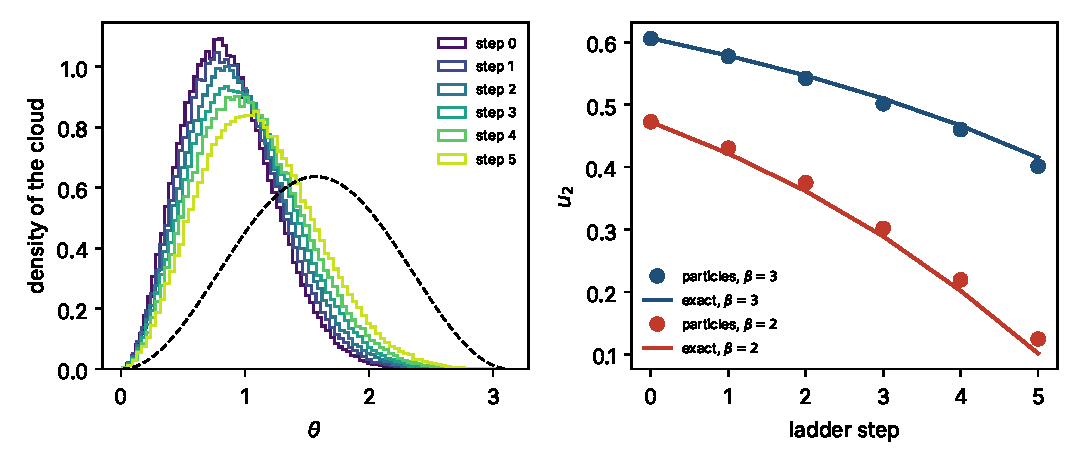
\includegraphics[width=0.75\textwidth]{figures/particle_mk.pdf}
\caption[The particle Migdal Kadanoff ladder]{The ladder run as a particle filter with $2\times10^5$ elements of SU(2), started from the heat kernel law. Left: the law of the rotation angle of the cloud over five steps from $\beta=3$, spreading toward the Haar density (dashed). Right: the second character coefficient of the cloud, points, against the exact flow, lines, from $\beta=3$ and $\beta=2$.}
\label{fig:particlemk}
\end{figure}

We implemented it (Figure~\ref{fig:particlemk}). With $2\times10^5$ particles, the density estimated from the first fourteen characters of the cloud, and $b=2$, the second character coefficient follows the exact flow to within $0.014$ over five steps from $\beta=3$ and to within $0.023$ from $\beta=2$. The errors grow along the ladder, as the error analysis of Section 20.4 of the Hilbert sixth book predicts for particle filters, because each update compounds the Monte Carlo error of the last.

The particle form needs no character expansion of the map, only samples and a density estimate, so it would apply to SU(3) and to block spin maps for which no closed recursion exists, subject to the accuracy of the density estimate at weak coupling and to degeneracy of the weights.

\section{What the Riemann Volumes Contribute}\label{ch:rhbooks}\index{Riemann Hypothesis}\index{de Bruijn Newman flow}\index{certified computation}\index{generalized gamma convolution}\index{Thorin measure}

This book is a sibling of our volumes \emph{Computing the Riemann Hypothesis}~\cite{PS26a,PS26b,PS26c}: Volume I, \emph{Representations of Xi, Thorin Measures and the Reciprocal Xi Function}; Volume II, \emph{Cauchy Deconvolution and Certified Computation}; and Volume III, \emph{Is There a Path?} Those volumes restate the Riemann Hypothesis as the positivity of a measure, the Thorin measure of a ratio of values of Riemann's $\Xi$ function, and they claim no proof. On 20 November 2026 L. Alp\"oge announced, with Lean code, a proof of the Riemann hypothesis and of the generalized Riemann hypothesis for Dirichlet $L$ functions~\cite{Alp26}. We have not examined it, and nothing in this book depends on it.

The programme starts from the reciprocal of Riemann's function $\xi(s)=\frac12s(s-1)\pi^{-s/2}\Gamma(s/2)\zeta(s)$, which is entire, satisfies $\xi(s)=\xi(1-s)$ and has Hadamard product $\xi(s)=\xi(0)\prod_\rho(1-s/\rho)$ over the zeros $\rho=\frac12+i\gamma$; the Riemann Hypothesis is the statement that every $\gamma$ is real. To the right of the zeros $1/\xi$ behaves like a Laplace transform, and one asks whether it is the Laplace transform of a generalized gamma convolution. The Euler product gives a L\'evy measure with atoms at $k\log p$ and the gamma factor a smooth part, so the question is the sign of a transported Thorin measure. Far to the right the Euler product converges absolutely and the Thorin structure is unconditional. At the centre of the strip the formal Thorin measure of the reciprocal is the sum of point masses at $\gamma^2/2$ over the zero ordinates: if the Riemann Hypothesis held, each would be a genuine point mass at a nonnegative location, and a zero off the line would move an atom to a complex location, where a nonnegative measure allows only nonnegative ones. The programme studies the family of Thorin measures indexed by the abscissa as a ladder, each descent a Cauchy or Poisson deconvolution that must preserve positivity.

Both problems have the form: a positive measure is given for free, and the hard statement is about where it lives.
\begin{center}
\small
\begin{tabular}{p{1.05in}p{1.5in}p{1.5in}}
\toprule
 & Riemann & Yang Mills \\ \midrule
free positivity & L\'evy measure of the reciprocal $\Xi$ law above the strip & spectral measure, by reflection positivity \\
transport & $2\sin^2$ lemma & $2\sin^2$ lemma \\
hard statement & Thorin measure nonnegative at level one half & Thorin densities decay at a uniform rate \\
ladder & levels $\alpha$ from one down to one half & couplings from strong to weak \\
obstruction & deconvolution without losing positivity & comparison without losing the gap \\
exactly solvable rung & Dedekind eta, P\'olya's function & two dimensions, hierarchical lattices \\
\bottomrule
\end{tabular}
\end{center}
The Hilbert sixth book puts it in one sentence, quoted in Section~\ref{ch:h6ym}: positivity is free and the support is hard.

\paragraph{\normalfont\scshape What we took.} The $2\sin^2$ lemma that drives Route B was found for the reciprocal $\Xi$ function, where it carries a L\'evy measure on the ordinates to a Thorin measure. In Section~\ref{ch:routeB} the same identity, applied to the spectral measure, gave the Thorin density as a L\'evy exponent and the gap as its decay rate. Nothing in the lemma knows which problem it is serving. Volume II studies the descent of the Thorin measure from level $\alpha$ to level $\alpha-\varepsilon$, a deconvolution that must preserve positivity; the gap estimator of Chapter~\ref{ch:estimation}, positive deconvolution with the gap as a support constraint, is the same inverse problem with the Laplace kernel in place of the Cauchy kernel. Finally the de Bruijn Newman flow~\cite{dB50}, treated in the Riemann volumes, deforms $\Xi$ by a backward heat equation and asks when all zeros are real. Theorem~\ref{thm:product} is a forward version on a compact group: under the heat flow on SU(2), the zeros of the heat kernel in the variable $\cos\theta$ are real, lie outside $[-1,1]$, and move outward monotonically, with Laguerre's theorem in place of the dynamics of the zeros of $\Xi$.

\paragraph{\normalfont\scshape What we give back.} Two things travel in the other direction. First, the equivalence theorem of Section~\ref{ch:routeB}: in a uniform Thorin inequality the constant is free, so a uniform bound with any constant implies the bound with constant one. The Riemann analogue, a statement that a weak positivity bound for the Thorin measure along the level ladder upgrades itself, is worth testing. Second, the lesson of the negative results: the ladder of this book, at $b=2$, is right at first order and wrong at second, and it misplaces the crossover by a constant shift. A deconvolution ladder for the Thorin measure can fail in the same two ways, correct local rate and wrong global constant, and the tests of Chapter~\ref{ch:progress} are a template for testing it against the known zeros.

The dependence is of method, not of result: nothing here assumes or uses any statement about the zeros of the zeta function.

\section{Sato Tate, Hecke Walks and the Langlands Volume}\label{ch:langlands}\index{Sato Tate law}\index{Langlands programme}\index{Ramanujan graph}\index{Selberg, A.}\index{Kesten McKay law}\index{Alon Boppana bound}\index{expander}\index{latent variable}\index{data augmentation}

Our volume \emph{On Langlands Conjectures: Probabilistic Methods}~\cite{PS26l} applies the Thorin framework to automorphic $L$ functions. Its objects look far from gauge theory. Several of them are not, and one of its negative results is the best statement we know of the difficulty of this book.

\subsection{Sato Tate is Haar measure on SU(2)}

The Sato Tate law $\frac1{2\pi}\sqrt{4-x^2}\,dx$ on $[-2,2]$ is the law of the trace $x=2\cos\theta$ of a Haar distributed element of SU(2): it is the weight $\frac2\pi\sin^2\theta\,d\theta$ of every integral in this book. The dictionary continues.
\begin{center}
\small
\begin{tabular}{p{0.44\textwidth}p{0.48\textwidth}}
\toprule
Langlands volume & this book \\ \midrule
Satake parameter of $\pi$ at $p$, a conjugacy class in SU(2) & holonomy of a plaquette, a conjugacy class in SU(2) \\
Sato Tate law, the limit over primes & Haar measure, the strong coupling limit \\
$L(s,\operatorname{Sym}^{n-1}\pi)$ and its moments & character coefficient $u_n$ of the plaquette law \\
Ramanujan Petersson: the parameter is unitary & the holonomy lies in the compact group \\
Hecke operator, a random walk on a tree & convolution on the group, decimation \\
Ramanujan graph: optimal spectral gap & mass gap \\
\bottomrule
\end{tabular}
\end{center}
The plaquette law at coupling $\beta$ is a tilt of Sato Tate by $e^{\beta x/2}$, and the heat kernel is its tilt by a theta function.

\subsection{A local factor in the heat kernel}

The Langlands volume gives a Thorin criterion for the Ramanujan Petersson conjecture at a prime: with Euler factor $E_p(w)=2\cosh(w\log p)-x_p$, the conjecture $|x_p|\le2$ holds if and only if $E_p(0)/E_p(\sqrt s)$ is the Laplace transform of a probability law, which is then a generalized gamma convolution. The same factor is in Chapter~\ref{ch:progress}. The Jacobi triple product writes the theta function of the SU(2) heat kernel as
\[
\vartheta(t,\theta)\ \propto\ \prod_{n\ge1}\Big(2\cosh\big(\tfrac{(2n-1)t}4\big)+2\cos\theta\Big),
\]
a product over $n$ of local factors of exactly this form, with $\log p$ replaced by $(2n-1)t/4$ and the Hecke eigenvalue $x_p$ by $-2\cos\theta$. The class angle is the Satake parameter, the same for every factor, and it is unitary because the holonomy is in SU(2). The heat kernel $K_t$ itself is a derivative of $\vartheta$ in the angle, and its own product, the one of Theorem~\ref{thm:product}, has factors $1+\cos\theta/\gamma_m(t)$ with $\gamma_m(t)$ between $\cosh((2m-1)t/4)$ and $\cosh((2m+1)t/4)$, so the Euler product reading is exact for the theta function and holds for $K_t$ only up to the position of the factors. Read through the Langlands volume, the SU(2) theta function is an $L$ function all of whose local factors satisfy Ramanujan, with the heat time as the variable that separates the primes.

\subsection{Ramanujan graphs}

A finite $(q+1)$ regular graph is Ramanujan if every eigenvalue of its adjacency matrix other than $\pm(q+1)$ has absolute value at most $2\sqrt q$. The bound of Alon and Boppana~\cite{Al86} says that no infinite family can do better: $2\sqrt q$ is the spectral radius of the universal cover, the $(q+1)$ regular tree, computed by Kesten~\cite{Kes59}, and McKay~\cite{McK81} showed that the eigenvalues of a large regular graph with few short cycles follow the spectral measure of the tree,
\[
\frac{(q+1)\sqrt{4q-\lambda^2}}{2\pi\big((q+1)^2-\lambda^2\big)}\,d\lambda\qquad\text{on }[-2\sqrt q,2\sqrt q].
\]
In the variable $x=\lambda/\sqrt q$ this tends to the Sato Tate law as $q\to\infty$. So the Kesten McKay law is a deformation of Haar measure on SU(2), with the degree as parameter, and a Ramanujan graph is a finite graph whose spectrum stays inside the support of that law. Lubotzky, Phillips and Sarnak~\cite{LPS88}, and Margulis, constructed such graphs from quaternion algebras, with the bound a consequence of the Ramanujan Petersson conjecture, Deligne's theorem~\cite{De74}.

Two features make them a model for the gap problem.

\paragraph{\normalfont\scshape A gap uniform in the volume.} The walk on a non bipartite Ramanujan graph has relaxation time at most $1/(1-\rho)$ with $\rho=2\sqrt q/(q+1)$, whatever the number of vertices. This is the property the mass gap asks of the lattice measure: a rate that does not degrade as the system grows. For the arithmetic Ramanujan graphs, the graph analogue of our problem is to prove it without Deligne.

\paragraph{\normalfont\scshape A duality with the group.} The walk on the group SU(2) has the representations as its spectrum: the heat kernel is $\sum_nn\,e^{-(n^2-1)t/4}\chi_n$. The walk on the representations has the group as its spectrum. Tensoring with the fundamental representation gives $\chi_2\chi_n=\chi_{n+1}+\chi_{n-1}$, and weighting by dimension gives the birth and death chain
\[
n\ \longrightarrow\ n\pm1\quad\text{with probability}\quad\frac{n\pm1}{2n}.
\]
Its eigenfunctions are $\sin(n\varphi)/n$ with eigenvalue $\cos\varphi$: the class angle of the group is the spectral parameter of the walk. This is, in the spectral sense, the regular tree at infinite degree, and the Hecke walk of the Langlands volume is its finite degree form.

\begin{proposition}[passage times on the representations]\label{prop:reppassage}
For the walk on the representations of SU(2) started at the trivial representation, in continuous time at rate one, the first passage time $T_N$ to the representation of dimension $N$ has the law of
\[
\sum_{j=1}^{N-1}\frac{E_j}{1-\cos(j\pi/N)}
\]
with independent standard exponential $E_j$: a generalized gamma convolution with Thorin atoms $1-\cos(j\pi/N)$. Its mean is $(N^2-1)/3$, which is $\frac43$ of the Casimir of the target.
\end{proposition}

\begin{proof}
With the state $N$ absorbing, the eigenfunctions are $\sin(n\varphi)/n$ with $\sin(N\varphi)=0$, so the Dirichlet rates are $1-\cos(j\pi/N)$ for $1\le j\le N-1$, and Keilson's theorem~\cite{Ke79} gives the representation. The mean is $\sum_j1/(1-\cos(j\pi/N))=\frac12\sum_j\csc^2(j\pi/2N)=(N^2-1)/3$.
\end{proof}

The script \texttt{code/spde\_extras.py} confirms the rates and the mean for $N=2$, $5$, $20$ and $100$. The proposition is the discrete companion of Proposition~\ref{prop:equator}: there, a passage on the group with rates $\frac12(4k^2-1)$ indexed by representations; here, a passage on the representations with rates indexed by angles. Brownian time $t$ on the group and the Casimir $n^2-1$ on its dual are conjugate, and the heat kernel coefficient $e^{-(n^2-1)t/4}$ is the pairing.

\subsection{Do latent variables help?}

The condition for Ramanujan at a prime is that a factor $2\cosh-x_p$ has its root in the right place. The product formula of the heat kernel has factors $1+x/\gamma_m$ with every $\gamma_m>1$, and that inequality has a probabilistic meaning: each factor is a two point mixture,
\[
1+\frac{x}{\gamma_m}=(1-p_m)\cdot1+p_m\,(1+x),\qquad p_m=\frac1{\gamma_m}\in(0,1).
\]

\begin{proposition}[a latent count for the heat kernel]\label{prop:latentcount}
Let $M_0=\sum_m\xi_m$ with independent Bernoulli variables $\xi_m$ of parameters $p_m=1/\gamma_m(t)$. Then
\[
\frac{K_t(\theta)}{K_t(\pi/2)}=\E\big[(1+\cos\theta)^{M_0}\big].
\]
Consequently, if $\theta$ has the heat kernel law, there is a latent count $M$, with $P(M=m)\propto P(M_0=m)\,C_{m+1}2^{-m}$ and $C_n$ the Catalan numbers, such that given $M$ the variable $y=\cos^2(\theta/2)$ has the Beta law with parameters $M+\frac32$ and $\frac32$. In particular $\E[\cos\theta\mid M]=M/(M+3)$, so that $e^{-3t/4}=\E\big[M/(M+3)\big]$.
\end{proposition}

\begin{proof}
Multiply out the product of Theorem~\ref{thm:product}. The Haar integral of $(1+\cos\theta)^m$ is $C_{m+1}2^{-m}$, and in the variable $y$ Haar measure is the Beta law with parameters $\frac32,\frac32$ and $(1+\cos\theta)^m=2^my^m$.
\end{proof}

The representation is exact and easy to use: draw $M$, then a Beta variable. The count has mean $0.20$, $1.0$, $2.9$ and $6.9$ at $\beta=\frac12$, $1$, $2$ and $4$, close to $2\beta-1$ at weak coupling (Figure~\ref{fig:langevinlatent}). The Wilson law has the same form with a Poisson count, since $e^{\beta x}=e^{-\beta}\sum_m\beta^m(1+x)^m/m!$. So both conjugate families of Section~\ref{ch:plgbc} lie in one family,
\[
\mathcal M=\big\{\,\E\big[(1+\cos\theta)^{M_0}\big]:\ M_0\ \text{a random nonnegative integer}\,\big\},
\]
and the latent count plays for class functions on SU(2) the part that the P\'olya Gamma variable~\cite{PSW13} plays for the logistic likelihood: it turns the density into a mixture of a conjugate kernel.

Does it help? In two ways.

\paragraph{\normalfont\scshape Bond moving becomes addition.} The $k$th power of $\E[(1+x)^{M_0}]$ is $\E[(1+x)^{M_0^{(1)}+\cdots+M_0^{(k)}}]$ with independent copies. The family $\mathcal M$ is closed under bond moving, and the update of the filter is the superposition of $k$ independent populations of size $M_0$.

\paragraph{\normalfont\scshape Decimation becomes coalescence.} Convolution on the group lowers the degree: $(1+x)^a*(1+x)^b$ is a polynomial of degree $\min(a,b)$. Normalise $f_a=(1+x)^a2^a/C_{a+1}$ to a probability density and write $f_a*f_b=\sum_jQ(j\mid a,b)\,f_j$. By Theorem~\ref{thm:coalescence} the coefficients $Q(j\mid a,b)$ are nonnegative for all $a,b$, with mean $ab/(a+b+2)$. In flat space two Gaussians of precisions $a$ and $b$ convolve to precision $ab/(a+b)$; the $2$ in the denominator is the curvature of the group in this language. Hence $\mathcal M$ is closed under convolution as well as under products, and the exact Migdal Kadanoff ladder, without projection, is a map on the laws of a nonnegative integer: superpose $b^{d-2}$ independent copies, then coalesce $b^2$ of the results in pairs with the kernel $Q$. The ladder is then an interacting particle system in the plainest sense, a population that is multiplied and then thinned, and confinement is its extinction: the count tends to zero, which is Haar measure.

So latent variables help here as they do elsewhere in our work: not by making a hard integral easy, but by exposing a conjugate structure in which the two operations of the ladder are addition and thinning.

\subsection{Spectral gaps that are theorems}

The Ramanujan graphs above, and Selberg's bound $\lambda_1\ge\frac3{16}$~\cite{Se65} on congruence quotients of the upper half plane, improved to $\lambda_1\ge\frac{975}{4096}$ by Kim and Sarnak~\cite{KS03} (Selberg's conjecture $\lambda_1\ge\frac14$ is open), are mass gaps in everything but name: spectral gaps uniform in the volume, deduced from Deligne's theorem and from bounds on Kloosterman sums and functoriality, not from curvature.

The moral for Yang Mills is uncomfortable and worth stating. In the two arithmetic cases above, the Ramanujan graphs and the congruence quotients, a gap uniform in the volume is known for a family of spaces built from SU(2) or its relatives, and the proof does not come from geometry or from probability. It comes from an extra structure, Hecke operators and the purity of Frobenius, that the lattice gauge theory does not obviously have. The nearest thing it has is the renormalisation group.

\subsection{The limitation theorem}

The opening chapter of the Langlands volume proves that no argument that sees only the limiting distribution of Frobenius data can detect automorphy: equidistribution is a consequence of functoriality and not a route to it. Sequences equidistributed for Sato Tate form a continuum; automorphic ones are countable.

We expect the gauge theory to have an analogue, which we do not prove, and we have met it several times without naming it. The law of a single plaquette, or of any finite set of loops, does not determine whether the theory has a gap: for any such law there are measures with and without exponential clustering that share it. The gap is a property of the joint law at all scales, as automorphy is a property of the sequence and not of its histogram.

\section*{Exercises}
\begin{enumerate}
\item Verify Kac's recursion (Chapter~\ref{ch:kacyang}) and check directly that $G_2$ has only real zeros.
\item Prove Asano's lemma for $c_0+c_1z_1+c_2z_2+c_3z_1z_2$.
\item Show that the partition function of one plaquette of U(1) lattice gauge theory is $I_0(\beta)$ and identify the hitting time of Proposition~\ref{prop:hitting}.
\item Verify the computation of Proposition~\ref{prop:groundstate} for the harmonic oscillator, which is not compact, so that the proposition does not cover it, and where $\mu$ is Gaussian and the diffusion is Ornstein Uhlenbeck.
\item Prove the Fourier bound for a class function law on SU(2) from Plancherel's theorem (Section~\ref{ch:h6}).
\item Expand $\frac{x}{\sinh x}\cdot2\cosh2x$ to second order and recover $\frac{11}{3}$.
\item For one plaquette, write the Langevin generator in the class angle and find the range of $\beta$ in which the Bakry \'Emery condition holds (Section~\ref{ch:spde}).
\item Compute $Q(\cdot\mid1,b)$ for every $b$ and verify the mean $b/(b+3)$ (Section~\ref{ch:langlands}).
\end{enumerate}
